\documentclass[a4paper]{article}
\addtolength{\hoffset}{-2.25cm}
\addtolength{\textwidth}{4.5cm}
\addtolength{\voffset}{-3.25cm}
\addtolength{\textheight}{5cm}
\setlength{\parskip}{0pt}
\setlength{\parindent}{0in}

%----------------------------------------------------------------------------------------
%	PACKAGES AND OTHER DOCUMENT CONFIGURATIONS
%----------------------------------------------------------------------------------------

\usepackage{blindtext} % Package to generate dummy text
\usepackage{charter} % Use the Charter font
\usepackage[utf8]{inputenc} % Use UTF-8 encoding
\usepackage{microtype} % Slightly tweak font spacing for aesthetics
\usepackage[portuguese]{babel} % Language hyphenation and typographical rules
\usepackage{amsthm, amsmath, amssymb} % Mathematical typesetting
\usepackage{float} % Improved interface for floating objects
\usepackage[final, colorlinks = true, 
            linkcolor = black, 
            citecolor = black]{hyperref} % For hyperlinks in the PDF
\usepackage{graphicx, multicol} % Enhanced support for graphics
\usepackage{xcolor} % Driver-independent color extensions
\usepackage{marvosym, wasysym} % More symbols
\usepackage{rotating} % Rotation tools
\usepackage{censor} % Facilities for controlling restricted text
\usepackage{listings, style/lstlisting} % Environment for non-formatted code, !uses style file!
\usepackage{pseudocode} % Environment for specifying algorithms in a natural way
\usepackage{style/avm} % Environment for f-structures, !uses style file!
\usepackage{booktabs} % Enhances quality of tables
\usepackage{tikz-qtree} % Easy tree drawing tool
\tikzset{every tree node/.style={align=center,anchor=north},
         level distance=2cm} % Configuration for q-trees
\usepackage{style/btree} % Configuration for b-trees and b+-trees, !uses style file!
\usepackage[backend=biber,style=numeric,
            sorting=nyt]{biblatex} % Complete reimplementation of bibliographic facilities
\addbibresource{ecl.bib}
\usepackage{csquotes} % Context sensitive quotation facilities
\usepackage[yyyymmdd]{datetime} % Uses YEAR-MONTH-DAY format for dates
\renewcommand{\dateseparator}{-} % Sets dateseparator to '-'
\usepackage{fancyhdr} % Headers and footers
\pagestyle{fancy} % All pages have headers and footers
\fancyhead{}\renewcommand{\headrulewidth}{0pt} % Blank out the default header
\fancyfoot[L]{} % Custom footer text
\fancyfoot[C]{} % Custom footer text
\fancyfoot[R]{\thepage} % Custom footer text
\newcommand{\note}[1]{\marginpar{\scriptsize \textcolor{red}{#1}}} % Enables comments in red on margin

%----------------------------------------------------------------------------------------


\begin{document}

\definecolor{dkgreen}{rgb}{0,0.6,0}
\definecolor{gray}{rgb}{0.5,0.5,0.5}
\definecolor{mauve}{rgb}{0.58,0,0.82}

\lstset{frame=tb,
  language=Java,
  aboveskip=3mm,
  belowskip=3mm,
  showstringspaces=false,
  columns=flexible,
  basicstyle={\small\ttfamily},
  numbers=none,
  numberstyle=\tiny\color{gray},
  keywordstyle=\color{blue},
  commentstyle=\color{dkgreen},
  stringstyle=\color{mauve},
  breaklines=true,
  breakatwhitespace=true,
  tabsize=3
}

\fancyhead[C]{}
\hrule \medskip
\begin{minipage}{0.295\textwidth}
\raggedright
\footnotesize
Bernardo Haab  \hfill\\
Luis Gois
\end{minipage}
\begin{minipage}{0.4\textwidth}
\centering
\large
Trabalho  Prático 1 - Meta 1\\
\normalsize
Redes de Comunicação\\
\end{minipage}
\begin{minipage}{0.295\textwidth}
\raggedleft
\today\hfill\\
\end{minipage}
\medskip\hrule
\bigskip

\newenvironment{itemize*}%
  {\begin{itemize}%
    \setlength{\itemsep}{0pt}%
    \setlength{\parskip}{0pt}}%
  {\end{itemize}}

\section{Introdução}

Este relatório apresenta as decisões feitas na implementação do projeto de compartilhamento de conteúdo entre professores e alunos. O projeto prevê algumas funcionalidades, divididas entre perfis de "administrador", "professor", e "aluno".

Aos administradores é atribuída a gerência de utilizadores, podendo adicionar, deletar, ou listar utilizadores. O administrador também pode desligar o servidor, impedindo que professores compartilhem conteúdos com seus alunos. Os professores possuem permissão para criar turmas, e enviar conteúdos a essas turmas. Aos alunos é permitido inscrever-se em turmas criadas por professores, e, a partir deste momento, os alunos passam a receber os conteúdos compartilhados pelos professores. Os alunos ainda podem verificar a turmas existentes, e quais está inscrito.

\section{Decisões arquiteturais}

O servidor é inicializado com o comando já especificado pelo professor:

\begin{verbatim}
    class_server {PORTO_TURMAS} {PORTO_CONFIG} {ficheiro configuração}
\end{verbatim}

Ao inicializar, o servidor utiliza o \textit{ficheiro configuração} para autenticar os usuários. Este ficheiro deve conter ao menos informações do perfil de 1 administrador, para que este possa acessar o sistema e criar os demais usuários. O acesso do administrador ao sistema é feito por meio de uma conexão  \textit{UDP} ao servidor, utilizando o comando \textit{netcat}. Para ter acesso liberado as funcionalidades disponíveis o administrador deve realizar login com os dados de um usuário cadastrado no \textit{ficheiro configuração}.

Usuários com perfil de professor e aluno devem acessar o sistema através do cliente desenvolvido. Para executar o cliente é utilizado o comando definido pelo professor:

\begin{verbatim}
    class_client {endereço do servidor} {PORTO_TURMAS}
\end{verbatim}

Estes usuários com perfil de professor podem realizar o envio de conteúdos para os alunos. Este compartilhamento é feito por meio de \textit{Multicast}. Para isso, a cada turma criada é atribuído um endereço \textit{Multicast}. Sendo assim, sempre que um professor deseja compartilhar um novo conteúdo precisa apenas informar o nome da turma, e o conteúdo que deseja enviar. O envio deste conteúdo para os alunos é feito pelo servidor.

O servidor ao receber a mensagem do tipo \textit{SEND} verifica se o cliente que enviou a requisição é um usuário autenticado com perfil de professor. Caso o cliente esteja autenticado corretamente, o servidor busca a turma em um local da memória compartilhada nomeado \textit{/classes}. Encontrando a turma desejada, o servidor inicia uma comunicação via \textit{socket Multicast} com o \textit{TTL} superior a 2, para garantir que a mensagem seja entregue a todos os dispositivos da rede configurada. Após emitir a mensagem desejada por este socket a conexão é encerrada.

Como citado acima, os dados referentes as turmas são armazenados pelo servidor em uma area de memória compartilhada, pois estes dados deve ser acessados por múltiplos processos. Cada cliente que deseja se comunicar como servidor realiza uma conexão \textit{TCP}, e o servidor passa a ouvir os comandos enviados em uma nova thread. Assim, as requisições de cada cliente é processada por uma thread nova no servidor. Então, para que a mesma turma criada pelo professor seja acessada por alunos este dado é armazenado em memória compartilhada.

% \section{Estrutura do Servidor}

Os processos realizados pelo servidor estão separados em duas grandes áreas no programa. As funcionalidades estão isolados conforme o protocolo utilizado, sendo assim, as funcionalidades de administrador acessadas via \textit{UDP} estão isoladas das demais que são acessadas via \textit{TCP}. Ao iniciar o servidor, dois processos são inicializados para lidar isoladamente com estas funcionalidades. Para isso, as funções de administração estão localizadas no ficheiro \(admin.c\), e tanto funções de alunos e professores  estão localizadas no ficheiro \(class.c\).

Destaca-se que, por conta da arquitetura criada para o projeto, o login é realizado por duas funções. A autenticação de administradores é feita separadamente da dos demais usuários. Com isso, é garantido que os administradores não podem acessar o sistema via \textit{TCP}, e alunos e professores não acessam via \textit{UDP}.

A execução do servidor pode ser vista na figura \ref{fig:servidor}. Com esta figura é possível verificar que o processo da administração (realizado no processo UDP) é feito separadamente do processamento de alunos e professores (realizado no processo TCP).

\begin{figure}
    \centering
    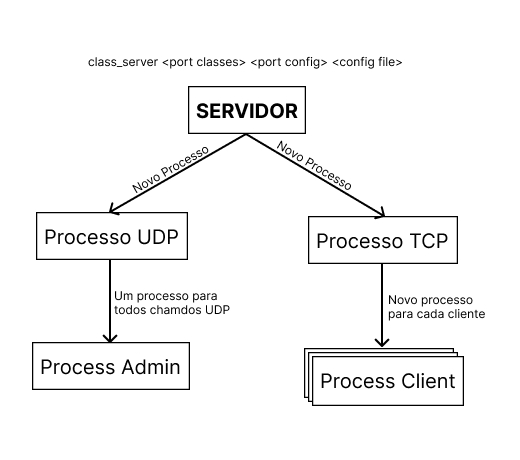
\includegraphics[width=0.5\linewidth]{img/Servidor.jpg}
    \caption{Execução do Servidor}
    \label{fig:servidor}
\end{figure}

A execução do programa cliente utilizado por professores e alunos pode ser vista na figura \ref{fig:cliente}. É possível verificar que após a inscrição em um turma uma nova thread é criada, responsável por receber conteúdos postados por professores. Esta arquitetura permite que os alunos possam seguir utilizando o sistema após inscrever-se em uma turma.

\begin{figure}
    \centering
    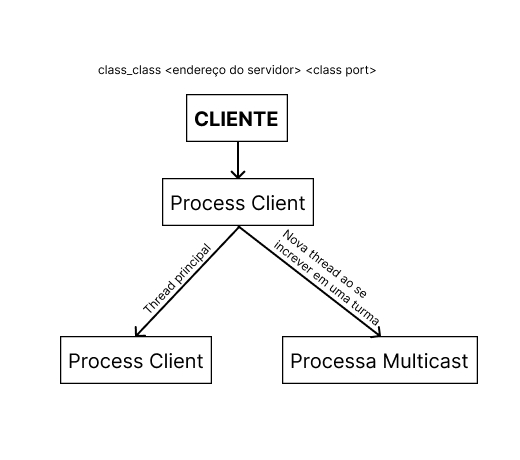
\includegraphics[width=0.5\linewidth]{img/Cliente.jpg}
    \caption{Execução do Cliente}
    \label{fig:cliente}
\end{figure}

Para que compilar este projeto no ambiente e permitir o teste no ambiente \textit{gns3} é utilizada a regra \textit{install} do arquivo Makefile. Esta regra compila os programas \textit{class\_server} e \textit{class\_client}, e os copia para todos os container utilizados no \textit{gns3},

% As funcionalidades descritas anteriormente são realizadas por um servidor desenvolvido. Assim, os usuários precisam se comunicar com o servidor para poder acessar o sistema. Usuários com perfil de administrador acessam o sistema diretamente por meio do comando \textit{netcat}.

% Como o administrador pode acessar as suas funções
% Como é feito o envio do conteúdo? O servidor envia



% \section{Descrição do ambiente GNS3}
% Os seguintes comandos foram utilizados para configurar o projeto GNS3. Foi também criada uma imagens docker nomeada 'project-server', a partir do arquivo Dockerfile que se encontra no diretório 'servidor'

% O servidor envia o conteúdo adicionado pelo professor para o multicast da turma.


%-----------------------------------------------------------------------


\end{document}
